\section{What is Scratch?}

\begin{frame}
    \bigcenter{What is Scratch?}
\end{frame}

% \begin{frame}\frametitle{What is Scratch?}
%     \begin{figure}
%         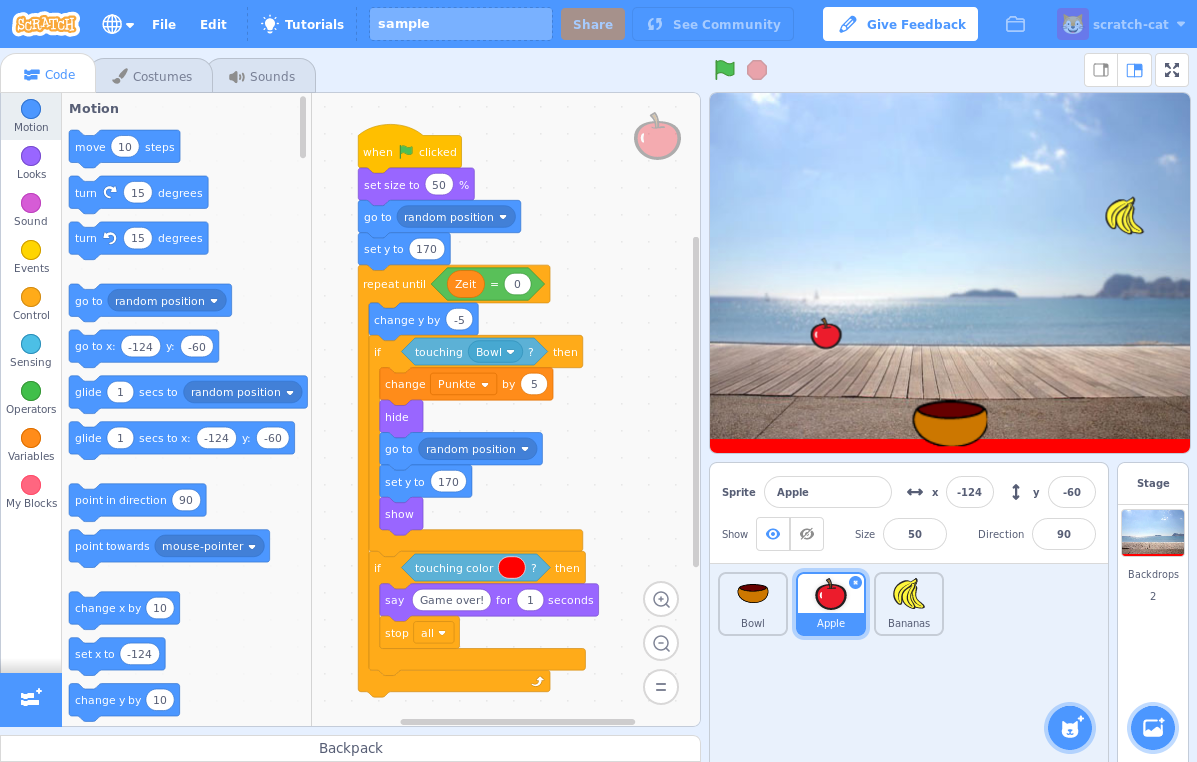
\includegraphics[width=.9\textwidth]{scratch-gui}
%         \caption{Scratch's GUI}
%     \end{figure}
% \end{frame}

\begin{frame}\frametitle{What is Scratch?}
    \begin{itemize}
        \item \textcolor{upfim}{Block-based} programming language
        \item Programs create \textcolor{upfim}{interactive animations} on a stage
        \item Code is separated into scripts that are triggered by events
        \item \greenflag event is the entry point of the program
    \end{itemize}
    \centering
    \medskip
    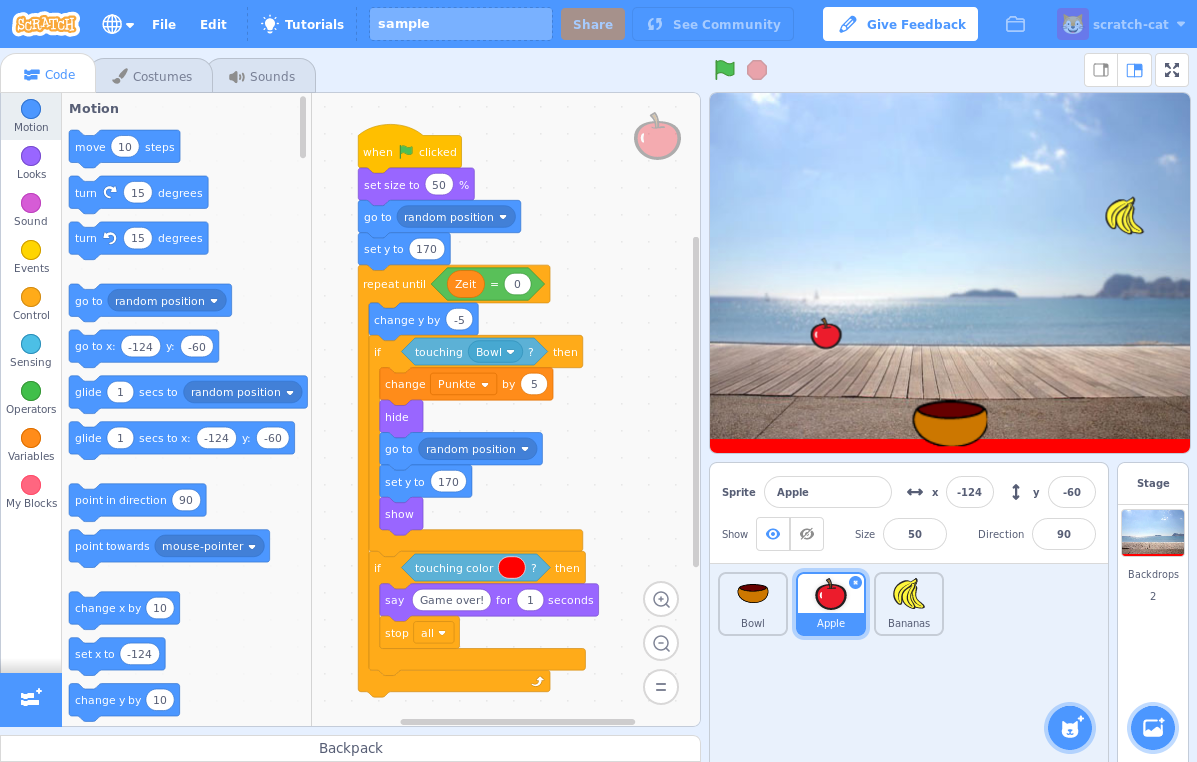
\includegraphics[width=.75\textwidth]{scratch-gui}
\end{frame}

% Scratch 3.0 is accessed through a web interface
% Code is made up of blocks that are chosen from a drawer and sticked together
% These blocks include statements, expressions, variables, control structures, and also something called hats
% Hats are used to trigger scripts through a variety of different events
% For example the "green flag" event is the entry point of the program, and other events include clicks, key presses and messages from other scripts
% These scripts manipulate sprites on a stage to create animations
% Scratch Programs are usually very interactive, Scratch has blocks to use keyboard and mouse input, which often makes for game-like programs

\section{Why automated testing for Scratch?}

\begin{frame}
    \bigcenter{Why automated testing for Scratch?}
\end{frame}

\begin{frame}\frametitle{Why automated testing for Scratch?}
    Many schools and universities deploy Scratch as a gentle introduction to programming.

    \pause
    \bigskip

    Grading Scratch assignments is very \textcolor{upfim}{time consuming}
    \begin{itemize}
        \item every project has to be opened individually
        \item programs require large amounts of \textcolor{upfim}{user interaction}
    \end{itemize}

    \pause
    \bigskip

    Some courses are attended by a \textcolor{upfim}{large number of students}
    \begin{itemize}
        \item manual testing for grading infeasible
        \item example University of Utah: $> 200$~\cite{itch}
    \end{itemize}

    \bigskip

    $\rightarrow$ Automated functional testing
%
%     \pause
%     \bigskip
%
%     Additionally, students can use automated tests to get feedback for their own implementations.
\end{frame}
